\chapter{自然数}

自然数集 $\mathbb{N}$ 是我们接触最早的数集,但就是这样一个“性质简单”的数集,我们也能从中发现一些有趣的东西。

\section{认识自然数}

自我们出生就一直和数字打交道:人有几根手指?河里有几只鸭子?朴素的我们掰着手指记数:0、1、2、3……10,至此我们会使用 0 到 10 的数字来计数了。

好像有什么不对劲,0 是自然数吗?

不同的书籍、领域给出的答案是不一样的,就根据 皮亚诺公理\footnote{参见 \href{https://zh.wikipedia.org/wiki/\%E7\%9A\%AE\%E4\%BA\%9A\%E8\%AF\%BA\%E5\%85\%AC\%E7\%90\%86}{维基百科}} 得出的结论,答案是肯定的。

这五条公理的内容如下:

\begin{itemize}
  \item $0$ 是自然数
  \item 每个自然数 $a$ 有且仅有一个后继数 $a'$ 为自然数
  \item 对自然数 $b$、$c$,当且仅当 $b' = c'$ 时有 $b = c$
  \item $0$ 不是任何自然数的后继数
  \item 任意有关自然数的命题,若其对自然数 $0$ 成立,且假定它对自然数 $a$ 为真时,可证其对 $a'$ 也成立,那么命题对所有自然数成立
\end{itemize}

个人认为把 0 认作自然数的好:离散数学中有单位元(幺元)的概念,若 $0 \notin \mathbb{N}$,则定义在集合 $\mathbb{N}$ 上的二元运算 $+$ 就没有单位元了,让其失去这样的性质就失去了数学的美感。

\section{四则运算}

\subsection{加法}

\subsection{减法}

\subsection{乘法}

\subsection{除法}

\subsubsection{取余}

\subsection{负数}

\subsection{奇数}

\subsection{偶数}

\subsection{因数}

\subsection{倍数}

\subsection{倒数}

\subsection{质数}

\subsection{合数}

\section{比较大小}

给出自然数 $a$、$b$,现在的我们看到不等式 $a > b$ 时,很容易就得到 $a - b > 0$,未免陷入到了代数的桎梏中——让我们回忆一下我们当初是怎么进行比较的:

\begin{center}
  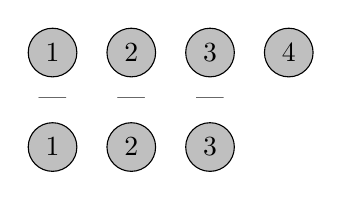
\begin{tikzpicture}
    \foreach \n/\t in
    {0/1,1/2,2/3,3/4}
    {\node[circle,fill=lightgray,draw]
    at (\n,1.2) {$\t$};}

    \foreach \n in
    {0,1,2}
    {\node at (\n,0.6) {|};}

    \foreach \n/\t in
    {0/1,1/2,2/3}
    {\node[circle,fill=lightgray,draw]
    at (\n,0) {$\t$};}
  \end{tikzpicture}
\end{center}

像这样 \strong{一一对应},直到一方比另一方多或相等。

为什么在这讲如此简单的东西呢?我们以一个数学问题切入感受一下:

Q:正奇数集 $O = \{1, 3, \cdots\}$ 与正偶数集 $E = \{2, 4, \cdots\}$ 哪个集合的元素个数(势)更大?

A:存在函数 $f: O \to E, f(x) = x + 1$ 为双射函数,则 $O, E$ 同势

而双射的定义如下:

若 $f: X \to Y$ 有 $\forall x \in X$ 存在唯一的 $y$ 与 $x$ 对应,且 $\forall y \in Y$ 存在唯一的 $x$ 与 $y$ 对应,则称 $f$ 为双射函数。换句话说,如果 $f$ 为两集合间的 \strong{一一对应} 关系,则 $f$ 是双射的。

在此也请读者们思考:

\begin{itemize}
  \item 上文中的 $O \cup E$ 与 $O, E$ 是否同势?若是请给出函数 $f$,否则给出理由。
  \item  集合 $A = \{x | 0 < x < 1, x \in \mathbb{R}\}$ 与集合 $\mathbb{R}$ 是否同势?若是请给出函数 $f$,否则给出理由。
\end{itemize}

\section{进制}

\section{平面图形}

\section{立体图形}

\section{统计}

\subsection{平均数}

\subsection{最值}

在一组数 $x_1, x_2, \cdots, x_n$ 中,若其中的某个数 $x_k$ 对其中任意一个数 $s$ 有 $x_k \geqslant s$,则称 $x_k$ 为最大值,同理可以给出最小值的定义。

那么根据这样的定义,最大值实际上是可以有“多个”的,比如一下一组数:$0, 1, 1, 2, 2$,实际上后两个数都是这组数的最大值,只是两者相同而已。

为了避免这样的重复,我们一般将这组数用一个集合表示,而集合中的元素只会出现一次,那么我们搬出严格定义如下:

设 $(P,\leqslant )$为偏序集,$S$ 为其子集。若 $g \in S$ 对任何 $s \in S$ 有 $s \leqslant g$,则 $g$ 称为 $S$ 的 \strong{最大元}(Greatest Element),同理若 $l \in S$ 对任何 $s \in S$ 有 $l \leqslant s$,则 $l$ 称为 $S$ 的 \strong{最小元}(Least Element)。

我们会用多种方式来表示最大值:如 $s_{\max}$、$\max{S}$,在元素个数为二时,我们还可以用一个算式来表达最大值:

记 $M = \max{\{a, b\}}$,则

$$M = \frac{a + b + |a - b|}{2}$$

容易证明 $a \geqslant b$ 时 $M = a$,$a < b$ 时 $M = b$。

同理记 $m = \min{\{a, b\}}$,则

$$m = \frac{a + b - |a - b|}{2}$$

由此我们就将比较抽象的取最大最小值用准确的算式表达出来了,在未来我们学习随机变量时会利用这个算式的。

\section{对称}

\section{角}

\section{坐标}

\section{鸡兔同笼}

4.认识物体和平面图形:长方体、正方体、圆柱和球等立体图形与长方形、正方形、三角形和圆等平面图形。

5.分类:单一标准的分类和不同标准的分类

6.6~9的认识和加减法:(1)6、7的认识和加减法(数数、数序、比大小、序数、写数、组成)。(2)8、9的认识和加减法(出现了“一图两式”和“一图四式”、渗透统计思想、比多比少内容)(3)10的认识和有关10的加减法(省略了10的序数意义、填未知加数)。(4)连加、连减和加减混合计算。(5)整理和复习。

7.11~20各数的认识:数数、读数、数序和大小、序数、写数、个位和十位、10加几和十几加减几(不退位)、十几减十。

8.认识钟表:认识钟面、认识整时、认识半时。

9.20以内的进位加法:9加几(“点数”、“接着数”、“凑十”和“根据具体题目选择特殊方法”),8、7、6加几(“拆小数,凑十数”、“拆大数,凑小数”和“交换加数的位置”),5、4、3、2加几和“用数学”。

一年级(下)

1.位置:用“上、下,前、后,左、右”描述物体的相对位置;根据行、列确定物体的位置。

2.20以内的退位减法:十几减9;十几减几;用数学。

3.图形的拼组:平面图形的特征;立体图形的关系

4.100以内数的认识 :数的认识(它包括:数数、数的组成、数位的含义、数的顺序)和加减(大小比较、整十数加一位数和相应的减法)。

5.认识人民币:认识人民币的单位元、角、分,知道1元=10角,1角=10分;简单的计算。

6.100以内的加法和减法(一):口算整十数加、减整十数;口算两位数加、减一位和整十数;用加法和减法解决简单的问题。

7.认识时间:认识几时几分(5分5分数、1分1分数)。

8.找规律:最简单的图形变化规律;稍复杂的图形变化规律;图形与数字变化规律;数字变化规律。

9.统计:简单的条形统计图(1格代表1);统计表;提出问题。

二年级(上)

1.长度单位:统一长度单位;认识厘米 用厘米量;认识米 用米量;认识线段,量、画线段。

2.100以内的加法和减法(二):两位数加两位数的不进位加法和进位加法;两位数减两位数的不退位减法、退位减法;连加、连减、加减混合运算和加减法估算。

3.角的初步认识:角和直角的初步认识。

4.表内乘法(一):乘法的初步认识;2~6的乘法口诀及乘加、乘减两步计算式题;用数学。

5.观察物体:从不同位置观察物体;轴对称;镜面对称。

6.表内乘法(二):7~9的乘法口诀;用7~9的乘法口诀解决简单的实际问题(求一个数的几倍是多少)。

7.统计:条形统计图(1格表示2个)。

8.数学广角:简单的排列(2个数字摆两位数);最简单的推理(2个条件);简单推理(3个条件)。

二年级(下)

1.数学问题:运用加法和减法两步计算解决问题,并学会使用小括号;运用乘法和加法(或减法)两步计算解决问题。

2.表内除法(一):除法的初步认识;用2~6的乘法口诀求商(被除数不超过12,被除数不超过36。);解决问题(用除法计算解决简单;用乘法和除法两步计算解决简单实际问题的内容)。

3.图形与变换:认识锐角和钝角;平移和旋转

4.表内除法(二):用7、8、9的乘法口诀求商;解决问题(求一个数是另一个数的几倍是多少;用乘、除法两步计算的稍复杂的实际问题)。

5.万以内数的认识:千以内数的认识(数数、读写、数的组成、大小比较);万以内数的认识(认识、读写、组成、数位顺序、中间有0的数的读写、比大小、近似数);口算整百整千数的加减。

6.克和千克:建立1克和1千克的观念、克和千克之间的进率、认识常见的秤、解决问题。

7.万以内的加法和减法(一):口算两位数加、减两位数(和在100以内),笔算几百几十加、减几百几十;加、减法估算。

8.统计:认识条形统计图(一格代表五个单位)和简单的复式统计表、合理预测。

9.找规律:图形的变化规律;数列的变化规律。

三年级(上)

1.测量:毫米、分米的认识、千米的认识和吨的认识。

2.万以内的加法和减法(二):加法、减法(两位数加两位数和是三位数的连续进位加法;三位数加、减三位数中连续进位加和连续退位减);加、减法的验算。

3.四边形:四边形和平行四边形的初步认识,周长的含义,长方形和正方形周长计算公式的探索和应用,对实物的估量等。

4.有余数的除法:意义和计算(表内除法竖式的含义;有余数除法竖式及余数的含义;余数和除数的关系);解决问题。

5.时、分、秒:时间单位“秒”,以及有关时间的简单计算。

6.多位数乘一位数:口算乘法(整十、整百数乘一位数的口算和相应的估算);笔算乘法(

7.分数的初步认识:几分之一、几分之几的认识,简单的分数加、减法(同分母加减、1减几分之几)。

8.可能性:事件发生的确定性和不确定性;可能发生的结果;事件发生的可能性有大小。

9.数学广角:两上衣和三裤子搭配的组合数;3个数字摆三位数的排列;4个队一共要踢多少场球的组合。

三年级(下)

1.位置与方向:辨认东、南、西、北、东北、西北、东南和西南八个方向,并认识简单的路线图。

2.除数是一位数的除法:口算除法(用一位数除商是整十、整百、整千的数、用一位数除几百几十或几千几百、除法估算);笔算除法;除法的验算;有关0的除法。

3.统计:简单的数据分析(横向条形统计图,起始格与其他格代表的单位量不一致);求平均数。

4.年、月、日:认识年月日;知道平年闰年;知道24时计时法;计算经过时间。

5.两位数乘两位数:口算;估算;笔算。

6.面积:面积和面积单位,长方形、正方形的面积计算,面积单位的进率,常用的土地面积单位。

7.小数的初步认识:认识小数(含义、读写法、大小比较);简单的小数加减法(一位小数的加减法)。

8.解决问题:乘法(或除法)、乘法和除法两步;乘加(减)、除减(加)两步计算解决问题。

9.数学广角:集合和等量代换。

四年级(上)

1.大数的认识:亿以内数的认识;亿以上数的认识;计算工具的认识及用计算器计算。

2.角的度量:认识射线和直线,知道线段、射线和直线的区别;认识常见的几种角,会比较角的大小,会用量角器量角的度数和按指定度数画角。

3.三位数乘两位数:口算乘法,笔算乘法,常见数量关系─速度、时间和路程,以及乘法的估算。

4.平行四边形和梯形:垂直与平行;平行四边形和梯形的认识。

5.除数是两位数的除法:口算除法、笔算除法。

6.统计:横、纵向复式条形统计图。

7.数学广角:合理安排(烙饼、沏茶、安排炒菜的顺序、码头卸货、田忌赛马)

四年级(下)

1.四则运算:解决问题(加减混合、乘除混合、两个商积之和差混合运算);三步式题;引导总结。

2.确定位置:根据方向、距离确定物体的位置;绘出物体的;位置关系的相对性;描述并绘制简单的线路图。

3.运算定律与简便计算:加法、乘法的交换律与结合律,乘法对于加法的分配律,以及这五条运算定律的一些比较简单的运用。

4.小数的意义和性质:小数的意义,认识小数的计数单位,会读、写小数,会比较小数的大小;小数的性质和小数点位置移动引起小数大小变化的规律;小数和十进复名数的相互改写;用“四舍五入法”保留一定的小数数位,求出小数的近似数,并能把较大的数改写成用万或亿作单位的小数。

5.三角形:三角形的特性、三角形两边之和大于第三边、三角形的分类、三角形内角和是180°及图形的拼组。

6.小数的加法和减法:小数加、减法、混合运算以及整数的运算定律推广到小数。

7.统计:折线统计图、

8.数学广角:植树问题

五年级(上)

1. 小数乘法:小数乘法;积的近似值;连乘、乘加、乘减两步计算;整数乘法运算定律推广到小数。

2. 小数除法:小数除以整数、一个数除以小数、商的近似值、循环小数、用计算器探索规律、解决问题(连除、去尾法、归一法)。

3. 观察物体:从不同的位置观察物体,所看到的形状是不同的;使学生能正确辨认从正面、侧面和上面观察到的简单物体或两个及一组立体图形的位置关系和形状。

4. 简易方程:用字母表示数和解简易方程,以及简易方程在解决一些实际问题中的运用。

5.多边形的面积:平行四边形的面积、三角形的面积、梯形的面积和组合图形的面积。

6. 统计与可能性:事件发生的等可能性以及游戏规则的公平性,会求简单事件发生的概率;理解中位数的意义,会求数据的中位数。

7. 数学广角:数字编码。

五年级(下)

1. 图形的变换:进一步认识图形的轴对称,探索图形成轴对称的特征和性质,学习在方格纸上画出一个图形的轴对称图形和画出一个简单图形旋转90°后的图形,发展空间观念。

2. 因数与倍数:因数、倍数;2、5、3的倍数的特征;质数、合数。

3. 长方体和正方体:长方体和正方体的认识,长方体和正方体的表面积,长方体和正方体的体积(容积)。

4. 分数的意义和性质:分数的意义、分数与除法的关系,真分数与假分数,分数的基本性质,最大公因数与约分,最小公倍数与通分以及分数与小数的互化。

5.分数的加法和减法:分数加、减法的意义,同分母分数加减法,异分母分数加减法,分数加减混合运算以及整数加法的运算定律推广到分数。

6. 统计:认识众数;复式折线统计图。

7. 数学广角:找次品。

六年级(上)

1. 位置:用数对确定位置。

2. 分数乘法:分数乘法、解决问题(求一个数的几分之几是多少)和倒数。

3. 分数除法:分数除法的意义与计算;解决问题;比的意义与基本性质,求比值与化简比,及其比的应用。

4. 圆:认识圆、圆的周长和圆的面积等。

5.百分数:百分数的意义和写法,百分数和分数、小数的互化以及用百分数解决问题。

6. 统计:体会扇形统计图的特点和作用。

7. 数学广角:“鸡兔同笼”问题

六年级(下)

1. 负数:初步认识负数,能正确的读、写正数和负数,知道0既不是正数也不是负数;用负数表示一些日常生活中的实际问题;比较正数、0和负数之间的大小。

2. 圆柱与圆锥:圆柱和圆锥的认识,圆柱的表面积,圆柱的体积和圆锥的体积。

3. 比例:比例的意义和基本性质;成正比例和反比例的意义;比例的应用。

4. 统计:综合应用学过的统计知识,能从统计图中准确提取统计信息,能够正确解释统计结果;根据统计图提供的信息,作出正确的判断或简单预测。

5. 数学广角:抽屉原理

6. 整理和复习:数与代数;空间与图形;统计与概率;综合应用。